%%%%%%%%%%%%%%%%% DO NOT CHANGE HERE %%%%%%%%%%%%%%%%%%%% {
\documentclass[12pt,letterpaper]{article}
\usepackage{fullpage}
\usepackage[top=2cm, bottom=4.5cm, left=2.5cm, right=2.5cm]{geometry}
\usepackage{amsmath,amsthm,amsfonts,amssymb,amscd}
\usepackage{lastpage}
\usepackage{enumerate}
\usepackage{fancyhdr}
\usepackage{mathrsfs}
\usepackage{xcolor}
\usepackage{graphicx}
\usepackage{subcaption}
\usepackage{listings}
\usepackage{hyperref}

\hypersetup{%
  colorlinks=true,
  linkcolor=blue,
  linkbordercolor={0 0 1}
}

\setlength{\parindent}{0.0in}
\setlength{\parskip}{0.05in}
%%%%%%%%%%%%%%%%%%%%%%%%%%%%%%%%%%%%%%%%%%%%%%%%%%%%%%%%%% }

%%%%%%%%%%%%%%%%%%%%%%%% CHANGE HERE %%%%%%%%%%%%%%%%%%%% {
\newcommand\course{CSI5138[F]: Intro: DL/RL}
\newcommand\semester{Fall 2019}
\newcommand\hwnumber{1}                 % <-- ASSIGNMENT #
\newcommand\NetIDa{Ao Zhang, 0300039680}           % <-- First Author
\newcommand\NetIDb{Lingfeng Zhang, 0300134245}           % <-- Second Author #
%%%%%%%%%%%%%%%%%%%%%%%%%%%%%%%%%%%%%%%%%%%%%%%%%%%%%%%%%% }

%%%%%%%%%%%%%%%%% DO NOT CHANGE HERE %%%%%%%%%%%%%%%%%%%% {
\pagestyle{fancyplain}
\headheight 35pt
\lhead{\NetIDa}
\lhead{\NetIDa\\\NetIDb}                 
\chead{\textbf{\Large Assignment \hwnumber}}
\rhead{\course \\ \semester}
\lfoot{}
\cfoot{}
\rfoot{\small\thepage}
\headsep 1.5em
%%%%%%%%%%%%%%%%%%%%%%%%%%%%%%%%%%%%%%%%%%%%%%%%%%%%%%%%%% }

\begin{document}

The code have two versions: one for TensorFlow, another for Numpy.

\section{Results without regularization}

Since there are $3$ changing parameters ($N$, $d$, and $\sigma$), we will focus on $1$ parameter each time in the following subsections with other fixing parameters. Some other training parameters are set as:
\begin{enumerate}
%    \item $\mathcal{D}_{test} = 2000$ and $\mathcal{D}_{bias} = 3000$;
    \item $\alpha_{learning} = 0.1$ with decay $0.96$ after each $100$ steps(learning rate decay);
    \item $epoches = 1000$ for iteratively updating loss function(convenient to compare different hyper-parameters because convergence condition is different).
\end{enumerate}

\subsection{Result of different complexities}

Complexity is researched first, the result is plotted as Figure~\ref{fig:complex_nonreg} shows,
\begin{figure}[h]
\centering
\begin{subfigure}{.45\textwidth}
  \centering
  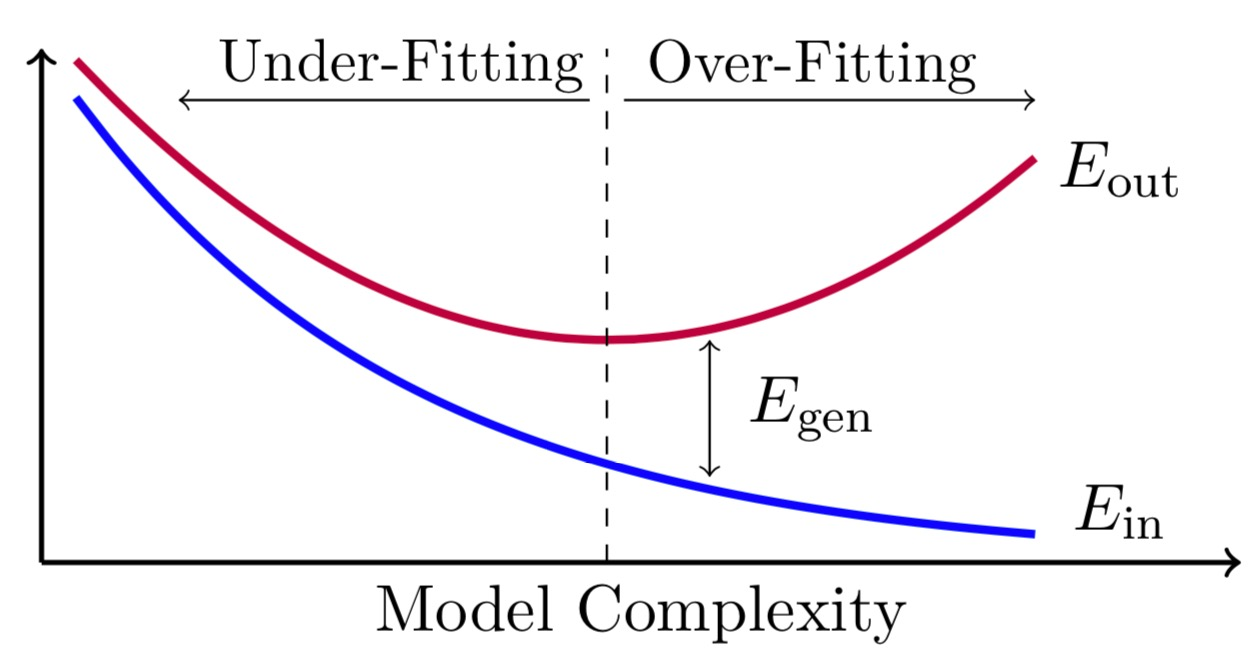
\includegraphics[width=.9\linewidth]{d_txtbook.jpg}
  \caption{\small figure from textbook}
  \label{fig:sub1}
\end{subfigure}%
\begin{subfigure}{.45\textwidth}
  \centering
  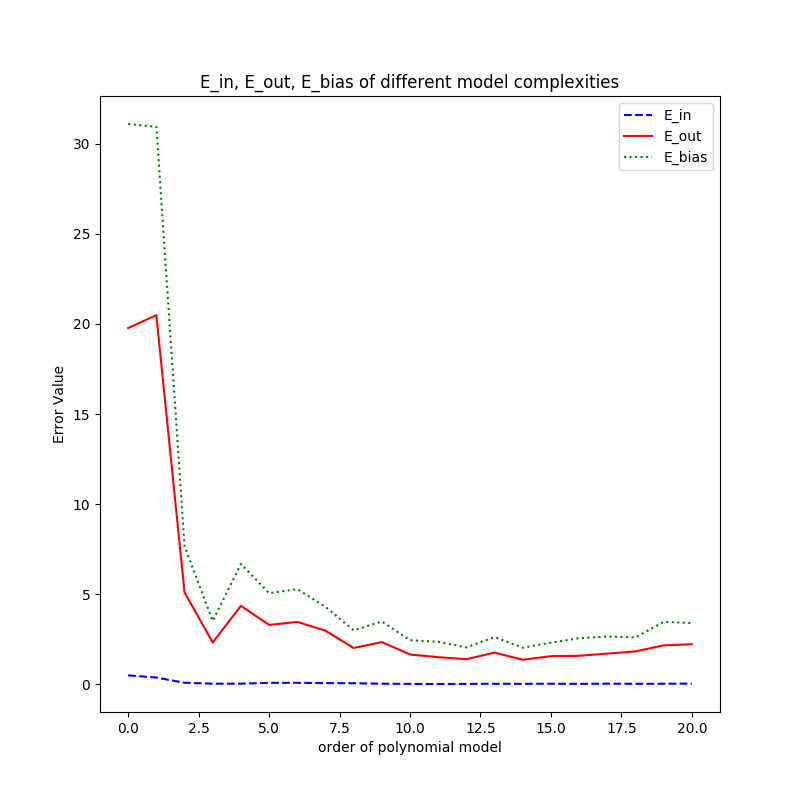
\includegraphics[width=.9\linewidth]{test_d_noreg.png}
  \caption{\small figure of test 1}
  \label{fig:sub2}
\end{subfigure}
\begin{subfigure}{.55\textwidth}
  \centering
  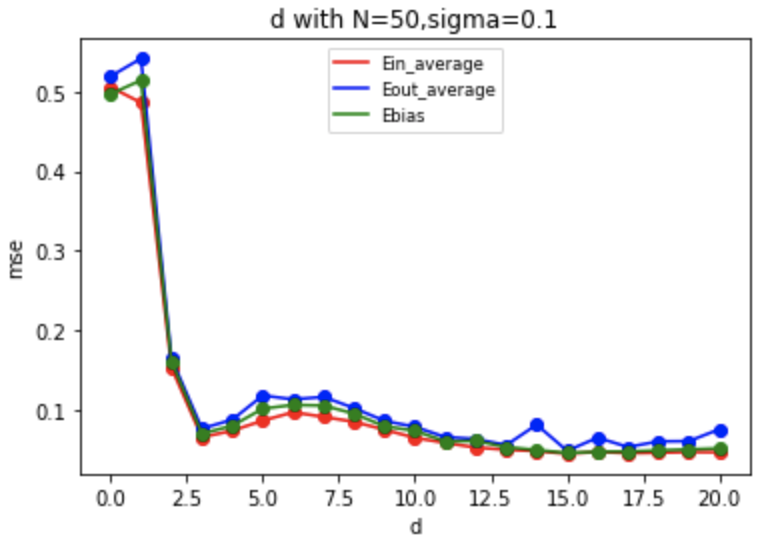
\includegraphics[width=.9\linewidth]{lzd50sig01.png}
  \caption{\small figure of test 2}
  \label{fig:sub3}
\end{subfigure}
\caption{\small Results of complexities.}
\label{fig:complex_nonreg}
\end{figure}

\subsubsection*{Parameters Settings}

\begin{itemize}
    \item Complexity $d$: $d \in \{ 1, 2, ..., 20 \}$;
    \item Dataset size $N$: $N = 50$;
    \item Variance $\sigma$: $\sigma = 0.1$.
\end{itemize}

\subsubsection*{Conclusion}

As the experiment shows, the result of the experiment basically follows what we learnt from the lecture. The out-sample error starts extremely high when the model is too simple to cover the dataset. A significant drop occurs after the complexity of the polynomial reaches around $1$ to $3$. The error gap ($E_{gen} = E_{out} - E_{in}$) reaches the minimal when the order becomes around $10 \sim 12$. And after that it goes up again. Thus, the over-fitting starts at order $12 \sim 15$ when the dataset size is $N = 50$.

The bias error $E_{bias}$ follows almost the same trend as the result of $E_{out}$.

When the model becomes more complex, Ein decreases, Eout decreases and then increases because the model from underfitting to fit well and then to overfitting, Egen increases. The complexity bound between underfitting model and overfitting model reaches best model in this case.

\subsection{Result of different sizes of dataset}

Then, dataset size is researched, the result is plotted as Figure~\ref{fig:size_nonreg} shows,
\begin{figure}[h]
\centering
\begin{subfigure}{.45\textwidth}
  \centering
  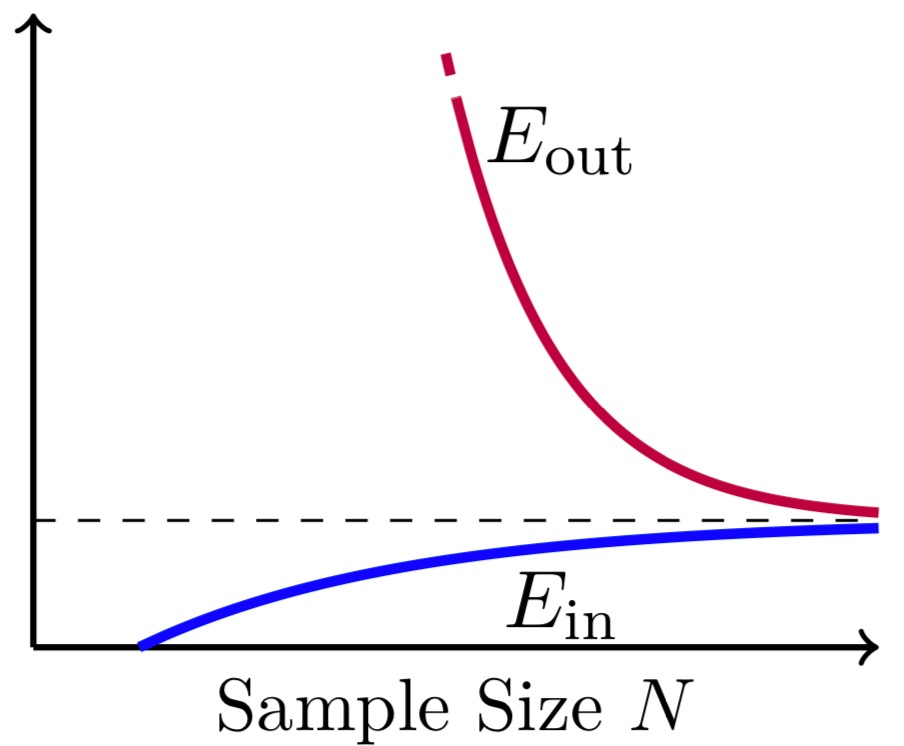
\includegraphics[width=.9\linewidth]{sample_txtbook.jpg}
  \caption{\small figure from textbook}
  \label{fig:sub1}
\end{subfigure}%
\begin{subfigure}{.45\textwidth}
  \centering
  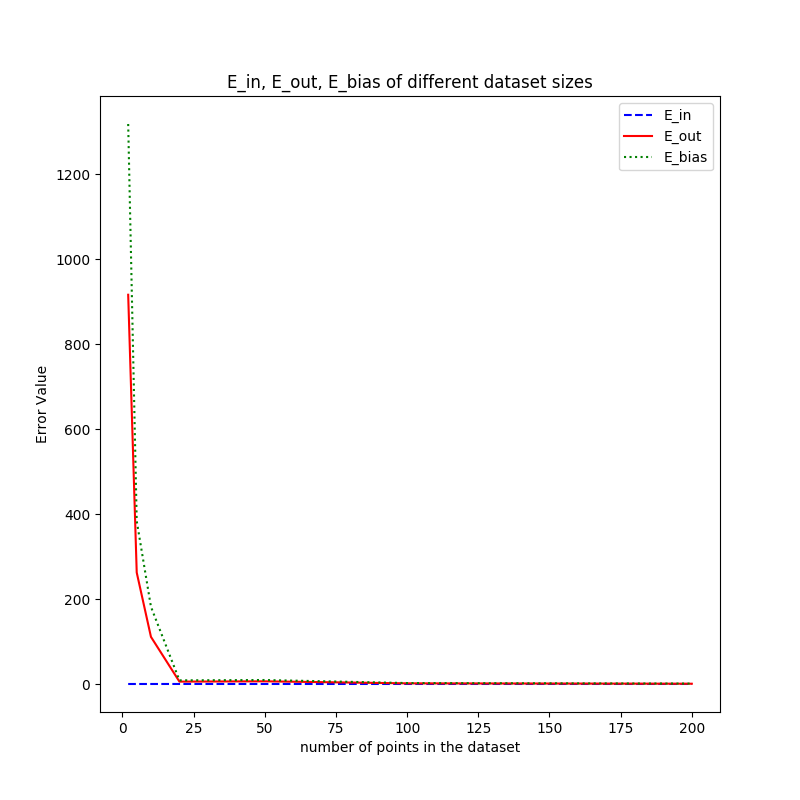
\includegraphics[width=.9\linewidth]{test_N_noreg.png}
  \caption{\small figure of test 1}
  \label{fig:sub2}
\end{subfigure}
\begin{subfigure}{.55\textwidth}
  \centering
  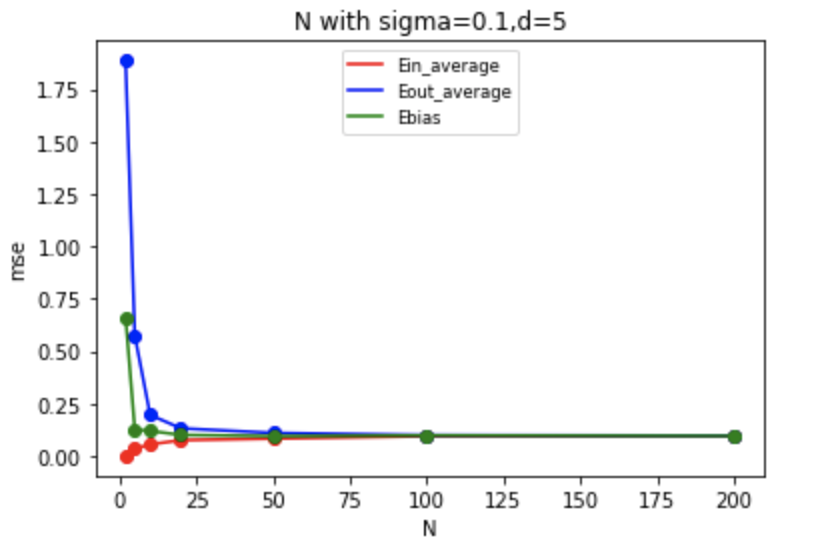
\includegraphics[width=.9\linewidth]{lzsig01d5.png}
  \caption{\small figure of test 2}
  \label{fig:sub2}
\end{subfigure}
\caption{\small Results of dataset size.}
\label{fig:size_nonreg}
\end{figure}

\subsubsection*{Parameters Settings}
\begin{itemize}
    \item Complexity $d$: $d = 5$;
    \item Dataset size $N$: $N \in \{ 2,5,10,20,50,100,200 \}$;
    \item Variance $\sigma$: $\sigma = 0.1$.
\end{itemize}

\subsubsection*{Conclusion}

As the experiment shows, the $E_{out}$ and $E_{bias}$ go all the way down and converge to a stable value just as the lecture slides indicate, although the converging speed is way faster than what we have learnt. The reason for that is the complexity of the model is only $d = 5$ points with small variance $\sigma = 0.1$

On the other hand, the $E_{in}$ increases slightly step-by-step, and finally reach the same level with $E_{out}$ and $E_{bias}$. This also follows the theory.

Overall, the conclusion is that the larger the dataset, the smaller error gap we could get, and the better result the model could learn.

\subsection{Result of different sizes of dataset in simple and complex model}

After, dataset size in both simple and complex model are researched, the result is plotted as Figure~\ref{fig:sig01d2/10} shows,

\begin{figure}[h]
\centering
\begin{subfigure}{.45\textwidth}
  \centering
  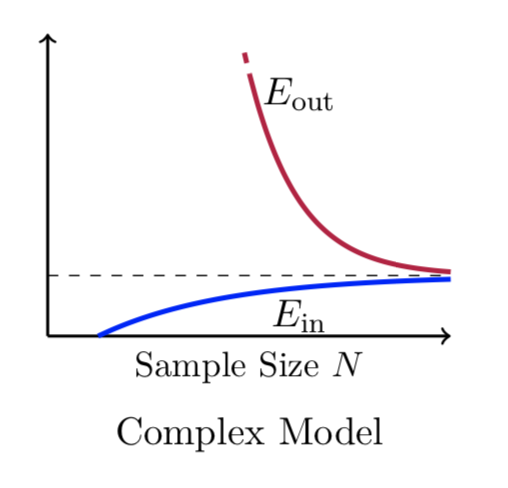
\includegraphics[width=.9\linewidth]{lectureComplexModel.png}
  \caption{\small more complex model in lecture slides}
  \label{fig:sub1}
\end{subfigure}
\begin{subfigure}{.45\textwidth}
  \centering
  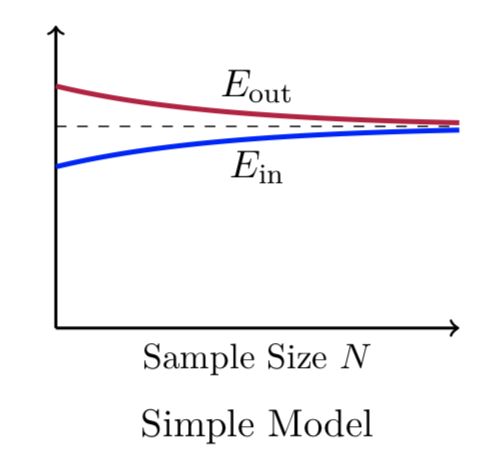
\includegraphics[width=.9\linewidth]{lectureSimpleModel.png}
  \caption{\small less complex model in lecture slides}
  \label{fig:sub2}
\end{subfigure}
\begin{subfigure}{.45\textwidth}
  \centering
  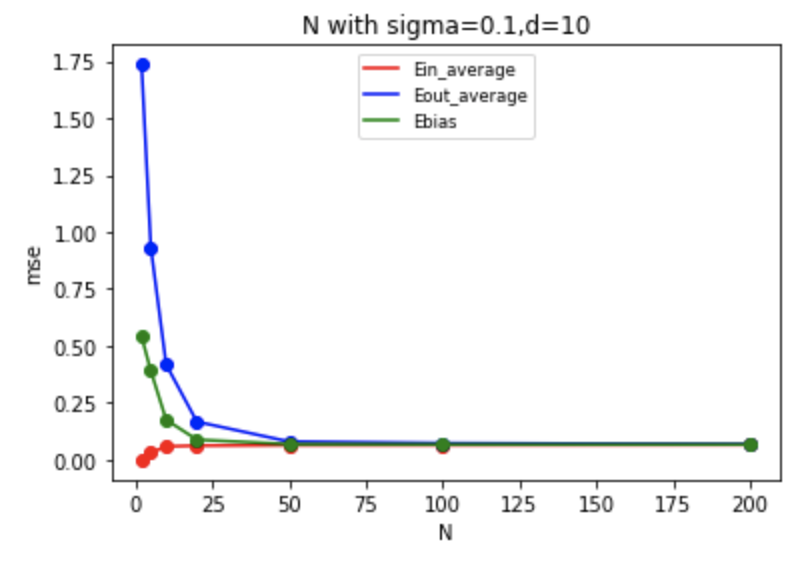
\includegraphics[width=.9\linewidth]{lzsig01d10.png}
  \caption{\small more complex model}
  \label{fig:sub3}
\end{subfigure}
\begin{subfigure}{.45\textwidth}
  \centering
  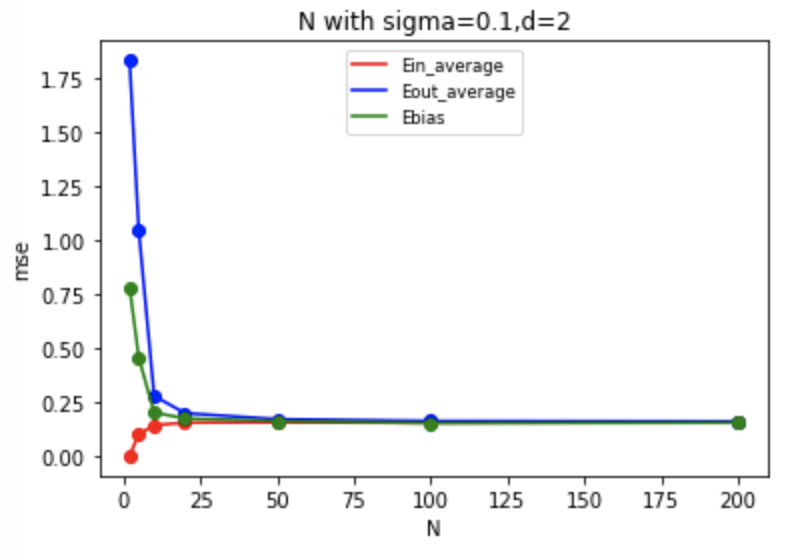
\includegraphics[width=.9\linewidth]{lzsig01d2.png}
  \caption{\small less complex model}
  \label{fig:sub4}
\end{subfigure}
\caption{\small different dataset size in $\sigma=0.1$ and 2/10-polynomial regression function without regularization}
\label{fig:sig01d2/10}
\end{figure}

\subsubsection*{Parameters Settings}
\begin{itemize}
    \item Complexity $d$: $d = 10$ more complex model, $d = 2$ less complex model;
    \item Dataset size $N$: $N = 200$;
    \item Variance $\sigma$: $\sigma \in \{ 0.01, 0.1, 1 \}$.
\end{itemize}

\subsubsection*{Conclusion}
As the experiment shows, both complex and simple model can converge with dataset size growing but higher MSE when convergence in simple model, as the lecture slides indicate. In lecture slides' plot(b) is part of the plot(d), starting from N around 10.

As for the plot(d) with 2-polynomial model(less complexity), When $N=2$, this simple model can fit the 2-point training data well and its in-sample error is 0. About the out-sample, testing sample size is 1000, the out-sample error will be extremely high because it is overfitting. With the increasing sample size, 2-polynomial model can not fit all training data well, so its in-sample error will increase, but the out-sample error will decrease because the overfitting decreases.If the sample size is large enough, in-sample error and out-sample error will be approximately equal(converged). This is because the noise points will disappear in extremely large dataset. 

Simple model(d) can not fit all large-size training data well. So both in-sample error and out-sample error are high. When the simple size increase, the in-sample error will increase and the out-sample error will decrease,finally they are converged.

Complex model‘s final converged error is lower than simple model because complex model can fit data better in large enough dataset. In general, the out-sample error is higher than in-sample error.

\subsection{Result of different dataset variance}

Then, dataset variance is researched, the result is plotted as Figure~\ref{fig:variance_nonreg} shows,
\begin{figure}[h]
\centering
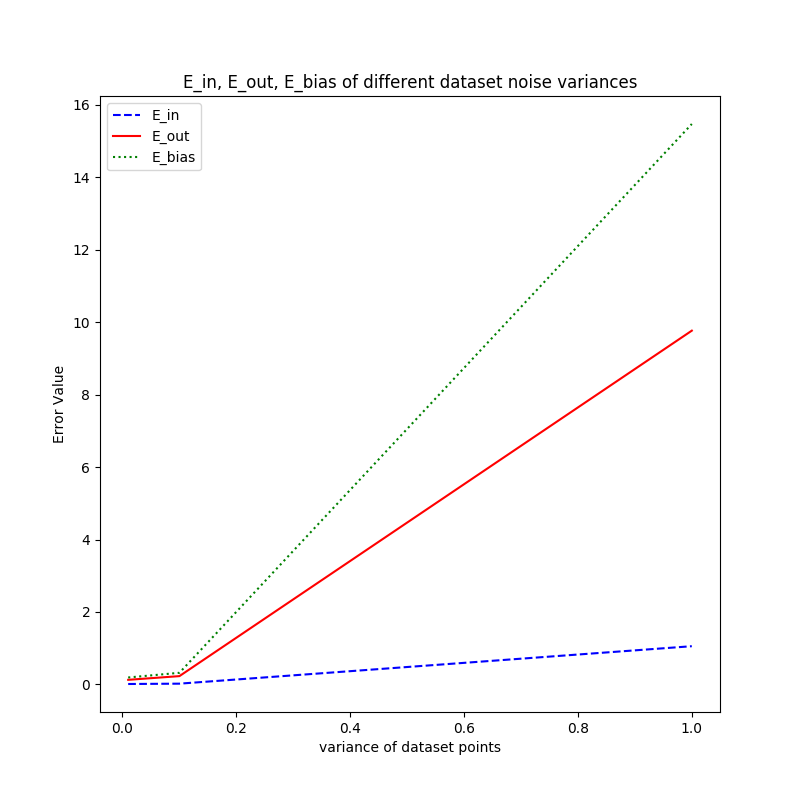
\includegraphics[width=.4\linewidth]{test_sigma_noreg.png}
\caption{\small Results of dataset variance.}
\label{fig:variance_nonreg}
\end{figure}

\subsubsection*{Parameters Settings}
\begin{itemize}
    \item Complexity $d$: $d = 10$;
    \item Dataset size $N$: $N = 200$;
    \item Variance $\sigma$: $\sigma \in \{ 0.01, 0.1, 1 \}$.
\end{itemize}

\subsubsection*{Conclusion}

As the experiment shows, all $E_{in}$, $E_{out}$ and $E_{bias}$ are dramatically increasing along with the dataset variance. Also, it is noticeable that $E_{bias}$ and $E_{out}$ are changing greater than $E_{in}$. This is due the fact that larger the variance is, more possible the model will be overfitted.

\section{Results with regularization}

Since we want to find the differences between regularized model and un-regularized model, in the following subsections, we keep all the parameters the same as the corresponding subsections above, and only introduce a new parameter $\lambda_{reg} = 0.01$. So, we will skip the \emph{parameters settings} part in the following subsections.

\subsection{Result of different model complexities}


\begin{figure}[h]
\centering
\begin{subfigure}{.45\textwidth}
  \centering
  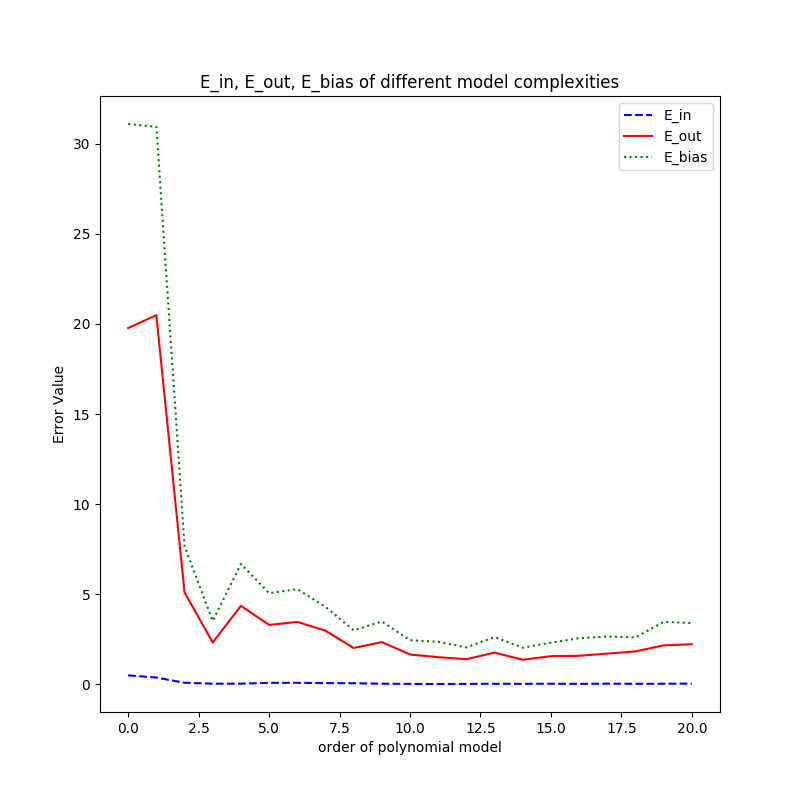
\includegraphics[width=.9\linewidth]{test_d_noreg.png}
  \caption{\small Un-regularized}
  \label{fig:sub1}
\end{subfigure}
\begin{subfigure}{.45\textwidth}
  \centering
  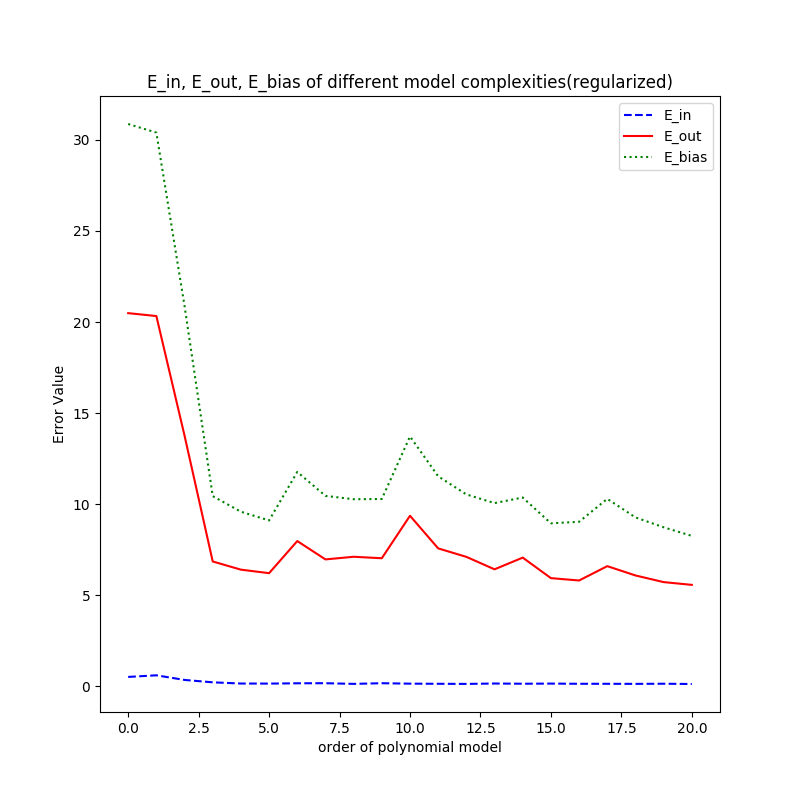
\includegraphics[width=.9\linewidth]{test_d_regularized.png}
  \caption{\small Regularized}
  \label{fig:sub2}
\end{subfigure}
\caption{\small Results of complexities.}
\label{fig:complex_reg}
\end{figure}

The result comparison between complexity curve before regularization and after regularization is shown as Figure~\ref{fig:complex_reg}.

\subsubsection*{Conclusion}

It is not hard to find out that after regularization, the value of the all the errors ($E_{in}$, $E_{out}$, and $E_{bias}$) are greater than those before. That is, because, an additional term is added into the loss function $\lambda_{reg} \cdot {\boldsymbol{ \theta} }^2$.

However, instead of bouncing back like un-regularized one, the regularized model keeps minimizing the errors even when the model becomes too complex, which shows more promising results when the model is over-parametrized.


\subsection{Result of different dataset sizes}

The comparison of results with dataset sizes between regularized model and un-regularized model is shown as Figure~\ref{fig:datasize_reg},
\begin{figure}[h]
\centering
\begin{subfigure}{.45\textwidth}
  \centering
  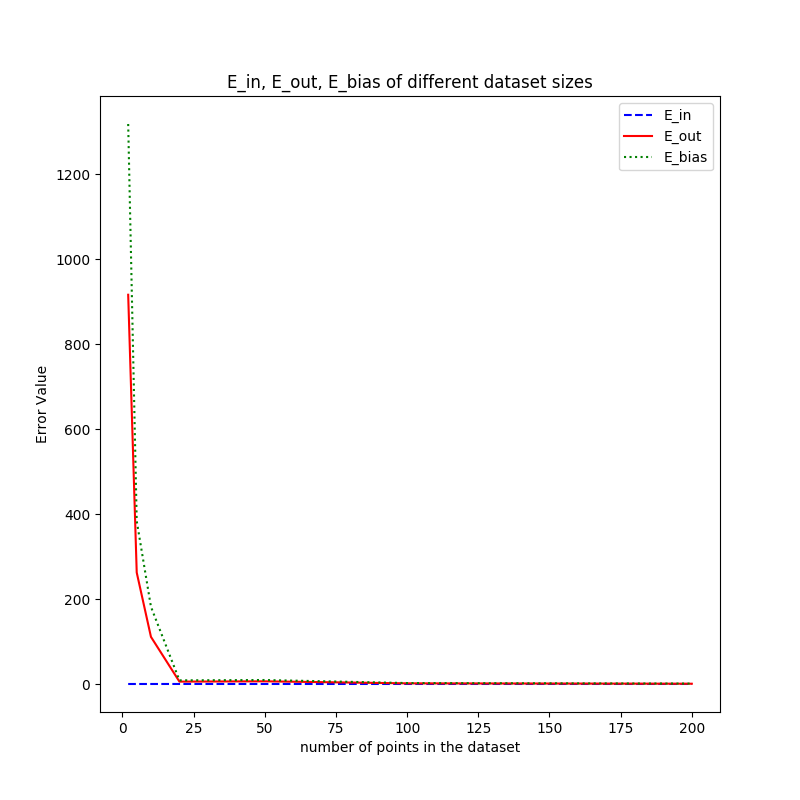
\includegraphics[width=.9\linewidth]{test_N_noreg.png}
  \caption{\small Un-regularized}
  \label{fig:sub1}
\end{subfigure}
\begin{subfigure}{.45\textwidth}
  \centering
  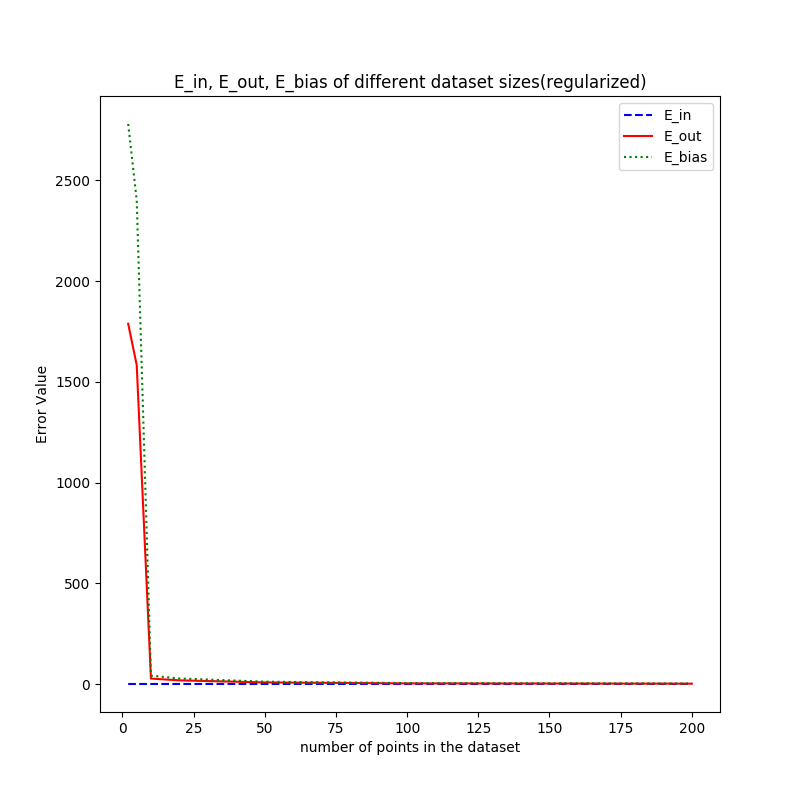
\includegraphics[width=.9\linewidth]{test_N_regularized.png}
  \caption{\small Regularized}
  \label{fig:sub2}
\end{subfigure}
\caption{\small Results of data sizes.}
\label{fig:datasize_reg}
\end{figure}

\subsubsection*{Conclusion}

As the two graphs show, the results have very similar characteristics, with all $E_{out}$ and $E_{bias}$ jumping down quickly and converge to the same value with $E_{in}$. A slight difference could be seen that the regularized model converge faster than the un-regularized one when the size of dataset is increasing.

Thus, we could say the regularized model could learn better than un-regularized one with the same dataset size.

\subsection{Result of different dataset variance}

The result comparison between dataset variance before regularization and after regularization is shown as Figure~\ref{fig:variance_reg},
\begin{figure}[h]
\centering
\begin{subfigure}{.45\textwidth}
  \centering
  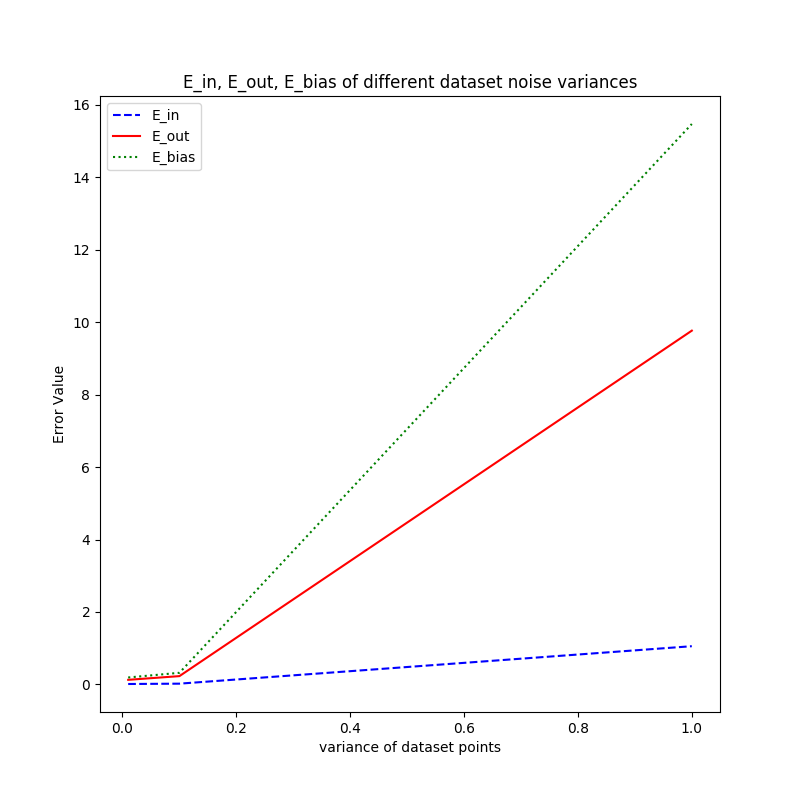
\includegraphics[width=.9\linewidth]{test_sigma_noreg.png}
  \caption{\small Un-regularized}
  \label{fig:sub1}
\end{subfigure}
\begin{subfigure}{.45\textwidth}
  \centering
  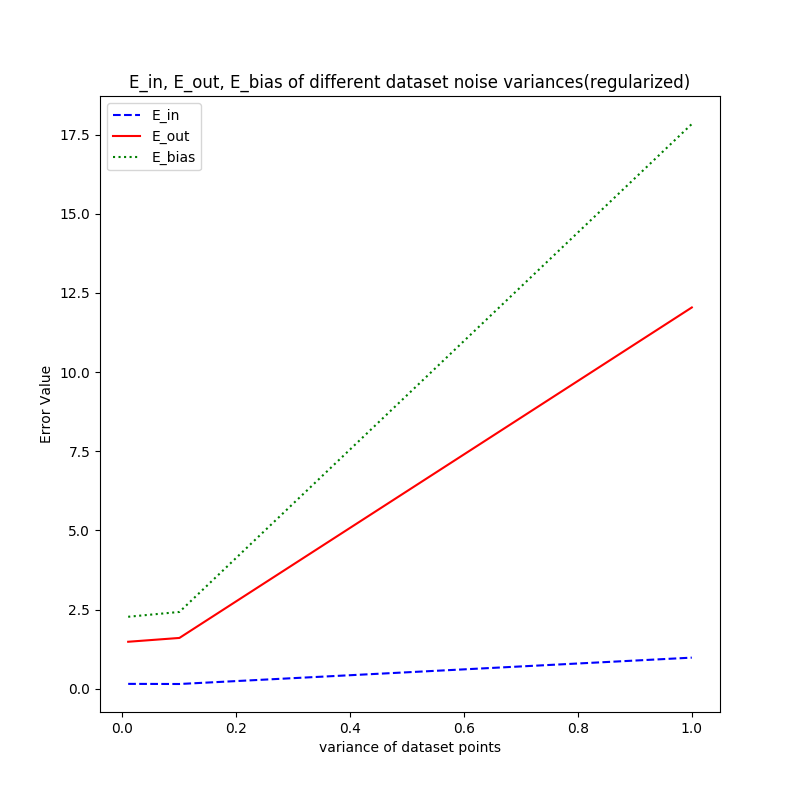
\includegraphics[width=.9\linewidth]{test_sigma_regularized.png}
  \caption{\small Regularized}
  \label{fig:sub2}
\end{subfigure}
\caption{\small Results of data vaiances.}
\label{fig:variance_reg}
\end{figure}

\subsubsection*{Conclusion}

Obviously, the influence of the dataset variance is independent to the regularization of the model.

Though it could be spotted that the errors of regularized model are greater than un-regularized one, it is mainly because of the additional term $\lambda_{reg} \cdot {\boldsymbol{ \theta} }^2$.

\subsection{Another way to illustrate regularization}

In this case, I used regularized value in 0.1. 

\begin{figure}[h]
\centering
\begin{subfigure}{.45\textwidth}
  \centering
  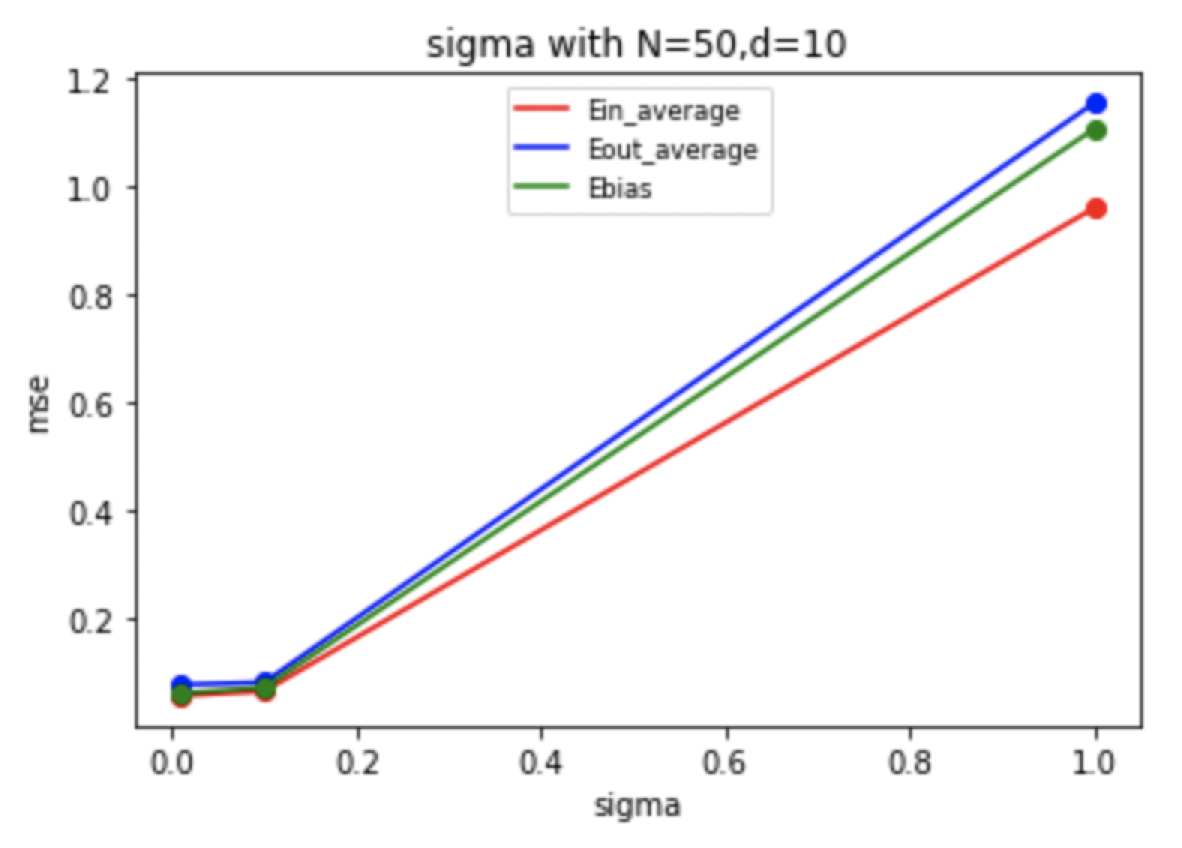
\includegraphics[width=.9\linewidth]{lzn50d10.png}
  \caption{\small Un-regularized}
  \label{fig:sub1}
\end{subfigure}
\begin{subfigure}{.45\textwidth}
  \centering
  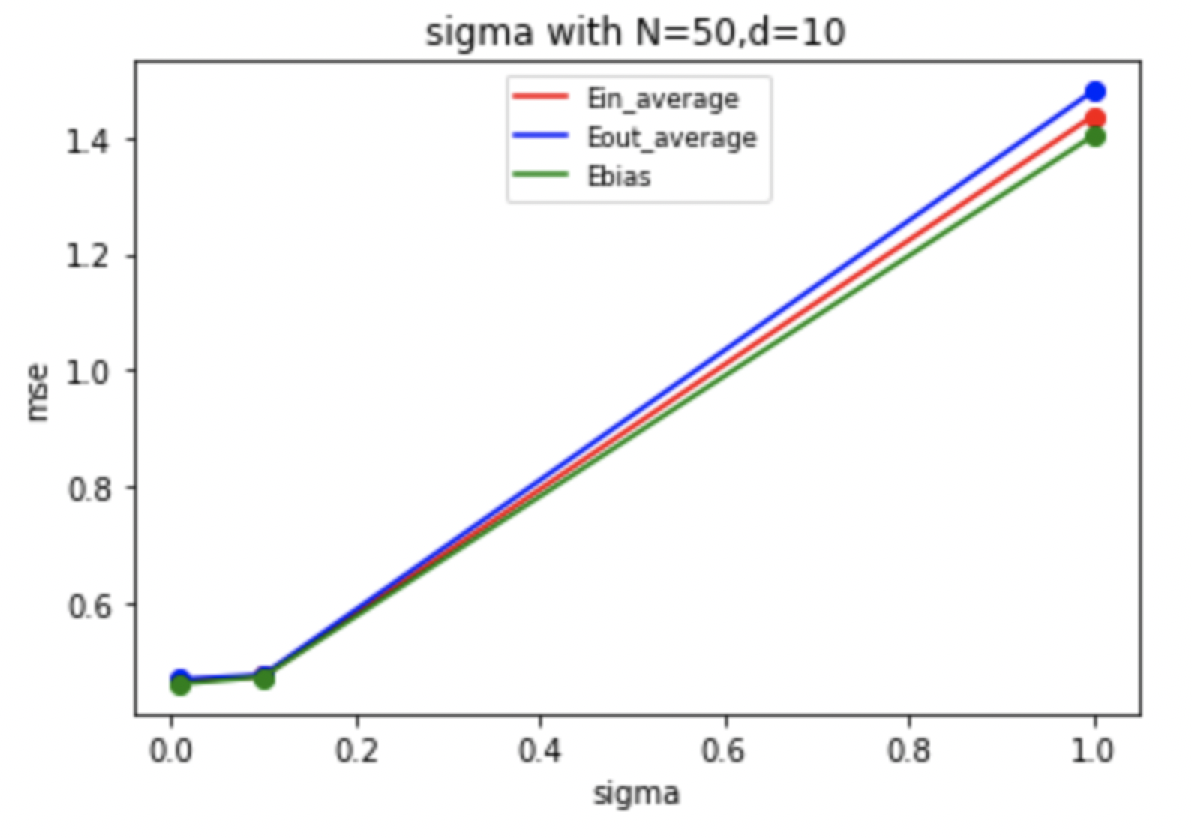
\includegraphics[width=.9\linewidth]{lzn50d10reg.png}
  \caption{\small Regularized}
  \label{fig:sub2}
\end{subfigure}
\caption{\small different $\sigma$ in 50 training data and 10-polynomial regression function}
\label{fig:n50d10}
\end{figure}

See Figure~\ref{fig:n50d10}, in un-regularized plot, at $\sigma$ = 1.0. We can see the regression model with 50 training data is overfitting because the difference between in-sample error and out-sample error is large. But at $\sigma=0.01$ and $\sigma=0.1$, the model fit well. This is because when $\sigma$ is small, the data is more mass, and less noisy. So the model can fit the data better in sample in-sample size data. Due to the sparsity at $\sigma=1$, the $E_{bias}$ can reduce the noise. So $E_{bias}$ is less than $E_{out}$.  

Since $\sigma=1$ is more sparse than $\sigma=0.1$ and the model is not complex enough, so the errors increase when $\sigma$ is growing. When the regression model is regularized in overfitting situation, the $E_{gen}=E_{out}-E_{in}$ will be decreased. Since I have not set the learning threshold to break out the iteration and just let the model do all iterations(be convenient to compare the difference of different hyper-parameter, because different models with different hyper-parameters reach different optimization), the parameter do the gradient descent slower in the regularization regression model. In the same iteration, regularized regression model learned slower, so the error in regularized regression model is larger than in un-regularized regression model. 

\begin{figure}[h]
\centering
\begin{subfigure}{.45\textwidth}
  \centering
  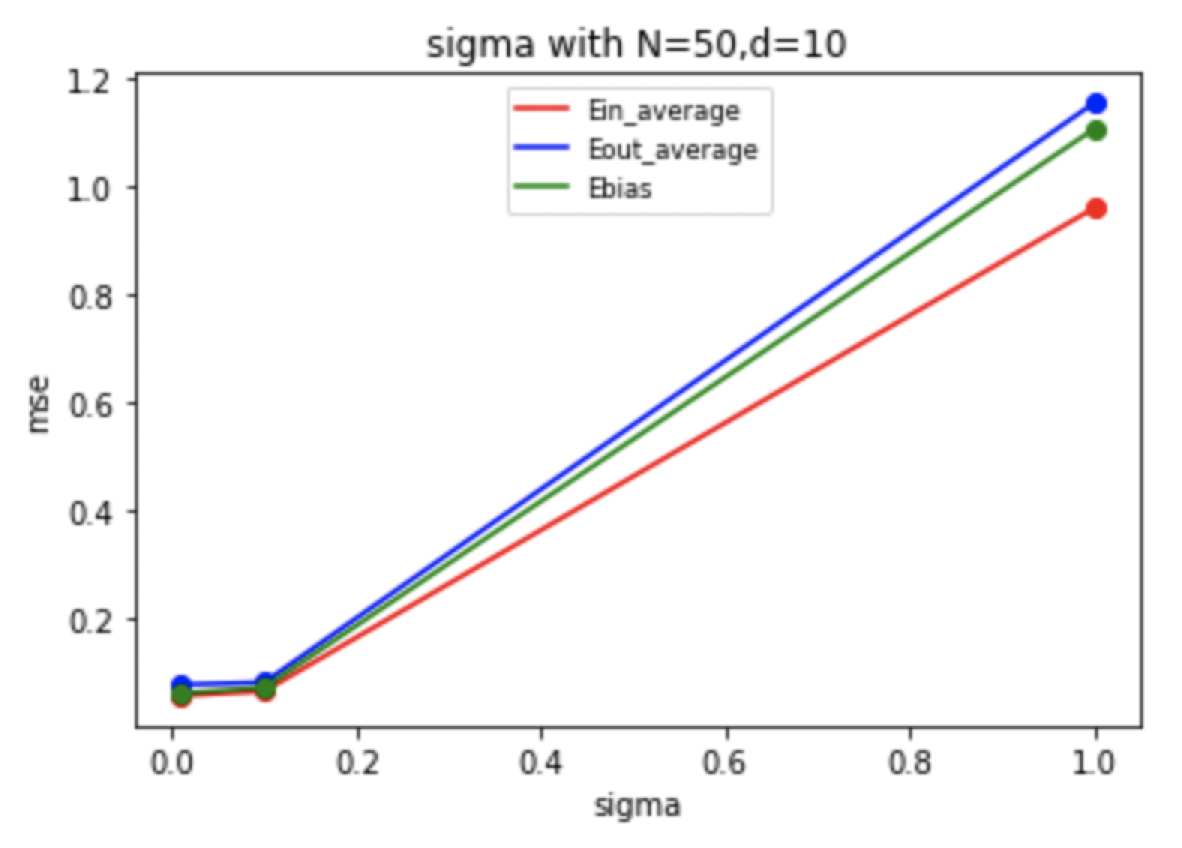
\includegraphics[width=.9\linewidth]{lzn50d10.png}
  \caption{\small small dataset}
  \label{fig:sub1}
\end{subfigure}
\begin{subfigure}{.45\textwidth}
  \centering
  \includegraphics[width=.9\linewidth]{lzn200d10.png}
  \caption{\small large dataset}
  \label{fig:sub2}
\end{subfigure}
\caption{\small different $\sigma$ in 50/100 training data and 10-polynomial regression function without regularization}
\label{fig:n50/200d10}
\end{figure}

See Figure~\ref{fig:n50/200d10}. In the regression model with same complexity, enlarging dataset can reduce overftting. Since two plots are generated in the same iteration times without iteration breaking condition, the training error in larger dataset is slightly larger than the training error in smaller dataset. 



\end{document}

